\documentclass[aspectratio=169]{beamer} % [mathserif]
\usepackage{amsmath}
\usepackage{graphicx}
\usepackage{subfigure}
\usepackage{wrapfig}
\usepackage{booktabs}
\usepackage{hyperref}
\usepackage{media9}
\usepackage{xcolor}
% \usepackage{pgfplots}
% \pgfplotsset{compat=1.18}
% \usepgfplotslibrary{dateplot}
% \usepackage{tipa}
% \usepackage{epstopdf} % this is needed for windows Texworks
\usepackage[absolute,overlay]{textpos} % ,showboxes

\setlength{\TPHorizModule}{1in}
\TPVertModule=\TPHorizModule

\DeclareGraphicsExtensions{.eps}

\usetheme{Marburg}
% \usetheme{Berkeley}
% \usecolortheme{rose}
\definecolor{naublue}{HTML}{002454}
\definecolor{nauyellow}{HTML}{FAC01A}
%\setbeamercolor{structure}{bg=nauyellow, fg=naublue}
\setbeamercolor{palette primary}{bg=nauyellow, fg=naublue}
\setbeamercolor{palette secondary}{bg=nauyellow, fg=naublue}
%%%% See https://en.wikibooks.org/wiki/LaTeX/Presentations#User-defined_themes
% \setbeamercolor{alerted text}{fg=orange}
% \setbeamercolor{background canvas}{bg=white}
% \setbeamercolor{block body alerted}{bg=normal text.bg!90!black}
% \setbeamercolor{block body}{bg=normal text.bg!90!black}
% \setbeamercolor{block body example}{bg=normal text.bg!90!black}
% \setbeamercolor{block title alerted}{use={normal text,alerted text},fg=alerted text.fg!75!normal text.fg,bg=normal text.bg!75!black}
% \setbeamercolor{block title}{bg=blue}
% \setbeamercolor{block title example}{use={normal text,example text},fg=example text.fg!75!normal text.fg,bg=normal text.bg!75!black}
% \setbeamercolor{fine separation line}{}
\setbeamercolor{frametitle}{fg=naublue}
% \setbeamercolor{item projected}{fg=black}
% \setbeamercolor{normal text}{bg=black,fg=yellow}
% \setbeamercolor{palette sidebar primary}{use=normal text,fg=normal text.fg}
\setbeamercolor{palette sidebar primary}{bg=naublue, fg=nauyellow}
% \setbeamercolor{palette sidebar quaternary}{use=structure,fg=structure.fg}
% \setbeamercolor{palette sidebar secondary}{use=structure,fg=structure.fg}
% \setbeamercolor{palette sidebar tertiary}{use=normal text,fg=normal text.fg}
\setbeamercolor{section in sidebar}{fg=nauyellow, bg=naublue}
\setbeamercolor{section in sidebar shaded}{fg=white}
% \setbeamercolor{separation line}{}
% \setbeamercolor{sidebar}{bg=red}
% \setbeamercolor{sidebar}{parent=palette primary}
% \setbeamercolor{structure}{bg=black, fg=green}
% \setbeamercolor{subsection in sidebar}{fg=brown}
% \setbeamercolor{subsection in sidebar shaded}{fg=grey}
\setbeamercolor{title}{fg=naublue}
% \setbeamercolor{titlelike}{fg=brown}

% \usepackage[latin1]{inputenc}

%%%% See https://en.wikibooks.org/wiki/LaTeX/Presentations#Title_page_and_author_information
\title[INF632 (EE499/EE599)]{Wearable Technologies and Applications\\(Wearable Informatics)} %
\author{Winfree}
\date{Lecture 9}
%\institute{Northern Arizona University}

%\logo{\includegraphics[width=.5in]{figures/logo}}
% \setbeameroption{show notes on second screen}

\begin{document}
	\maketitle


% \section[Outline]{}
% \frame{\tableofcontents}

\section{Model Evaluation}
	\subsection{Importance of Evaluating Model Performance}
	\begin{frame}
		\frametitle{Importance of Evaluating Model Performance}
		Evaluating model performance is crucial in the development and deployment of machine learning models. It ensures that the model serves its intended purpose effectively.
		\begin{itemize}
			\item Model Effectiveness
			\begin{itemize}
				\item Performance evaluation helps determine how well the model predicts outcomes compared to actual values.
				\item Metrics like accuracy, precision, recall, and F1 score provide quantifiable measures of how well the model performs.
			\end{itemize}
			\item Model Generalizability
			\begin{itemize}
				\item Evaluating performance on unseen data (e.g., validation/test sets) helps identify whether a model has learned the training data too well, potentially leading to poor performance on new data.
				\item Techniques such as k-fold cross-validation give insights into how well the model generalizes to independent datasets.
			\end{itemize}
			\item ...
		\end{itemize}
	\end{frame}
	\begin{frame}
		\frametitle{Importance of Evaluating Model Performance}
		Evaluating model performance is crucial in the development and deployment of machine learning models. It ensures that the model serves its intended purpose effectively.
		\begin{itemize}
			\item ...
			\item Identifying Areas for Improvement
			\begin{itemize}
				\item Performance evaluation can highlight specific areas where the model struggles, such as certain classes or conditions. This insight can direct further data collection and feature engineering.
				\item Understanding which metrics are lacking can help in adjusting model parameters, choosing different algorithms, or refining the features used for training.
			\end{itemize}
			\item Guiding Decision-Making
			\begin{itemize}
				\item Evaluation metrics can guide the selection among different modeling approaches based on their performance in the context of the problem.
				\item Specific metrics, such as recall in medical diagnoses, are more meaningful in certain applications than general accuracy, guiding stakeholders in business decisions.
			\end{itemize}
		\end{itemize}
	\end{frame}

\section{True and False Positives and Negatives}
	\begin{frame}
	\frametitle{What did we get right? And wrong?}
		Let's start with the idea of counting the observations that we got correct, and counting those that we got incorrect.

		But it's more than just that.  We have two ``correct'' conditions, and two ``incorrect'' conditions.

		Let's consider just testing a model that detected something to be present or not.  Medical conditions often fit this example.
	\end{frame}
	\subsection{True Positive}
	\begin{frame}
	\frametitle{True Positive}
		\begin{center}
			\begin{tabular}{|c|c|c|}
				\hline
				& \textbf{Predicted Positive} & \textbf{Predicted Negative} \\
				\hline
				\textbf{Actual Positive} & {\color{blue}True Positive (TP)} & False Negative (FN) \\
				\hline
				\textbf{Actual Negative} & False Positive (FP) & True Negative (TN) \\
				\hline
			\end{tabular}
		\end{center}

		{\bf True Positives (TP)} refer to the instances where the model correctly predicts the positive class. In other words, these are cases where the actual class was positive, and the model also predicted it as positive.

	\end{frame}
	\subsection{True Negative}
	\begin{frame}
	\frametitle{True Negative}
		\begin{center}
			\begin{tabular}{|c|c|c|}
				\hline
				& \textbf{Predicted Positive} & \textbf{Predicted Negative} \\
				\hline
				\textbf{Actual Positive} & True Positive (TP) & False Negative (FN) \\
				\hline
				\textbf{Actual Negative} & False Positive (FP) & {\color{blue}True Negative (TN)} \\
				\hline
			\end{tabular}
		\end{center}

		{\bf True Negatives (TN)} refer to the instances where the model correctly predicts the negative class. In other words, these are cases where the actual class was negative, and the model also predicted it as negative.
	\end{frame}

	\subsection{False Positive}
	\begin{frame}
		\frametitle{False Positive}
		\begin{center}
			\begin{tabular}{|c|c|c|}
				\hline
				& \textbf{Predicted Positive} & \textbf{Predicted Negative} \\
				\hline
				\textbf{Actual Positive} & True Positive (TP) & False Negative (FN) \\
				\hline
				\textbf{Actual Negative} & {\color{blue}False Positive (FP)} & True Negative (TN) \\
				\hline
			\end{tabular}
		\end{center}

		{\bf False Positives (FP)} are instances where the model incorrectly predicts the positive class. These are cases where the actual class was negative, but the model predicted it as positive.
	\end{frame}

	\subsection{False Negative}
	\begin{frame}
		\frametitle{False Negative}
		\begin{center}
			\begin{tabular}{|c|c|c|}
				\hline
				& \textbf{Predicted Positive} & \textbf{Predicted Negative} \\
				\hline
				\textbf{Actual Positive} & True Positive (TP) & {\color{blue}False Negative (FN)} \\
				\hline
				\textbf{Actual Negative} & False Positive (FP) & True Negative (TN) \\
				\hline
			\end{tabular}
		\end{center}

		{\bf False Negatives (FN)} are instances where the model incorrectly predicts the negative class. These are cases where the actual class was positive, but the model predicted it as negative.
	\end{frame}

\section{Confusion Matrix}
	\subsection{Structure}
	\begin{frame}
		\frametitle{Structure}
		The table we were just looking at is known as a Confusion Matrix.  You can picture this as raw numbers, or as percentages.

		\begin{center}
			\begin{tabular}{|c|c|c|}
				\hline
				& \textbf{Predicted Positive} & \textbf{Predicted Negative} \\
				\hline
				\textbf{Actual Positive} & 53 & 47 \\
				\hline
				\textbf{Actual Negative} & 26 & 74 \\
				\hline
			\end{tabular}
		\end{center}
	\end{frame}

	\subsection{More than Two Classes}
	\begin{frame}
		\frametitle{More than Two Classes}
		But those examples are all assuming True/False classification.  If we have more classes, we simply add rows and columns.

		\begin{center}
			\begin{tabular}{|c|c|c|c|c|}
				\hline
				& \textbf{Predicted A} & \textbf{Predicted B} & \textbf{Predicted C} & \textbf{Predicted D}\\
				\hline
				\textbf{Actual A} & TP(A) & FN(A, B) & FN(A, C) & FN(A, D) \\
				\hline
				\textbf{Actual B} & FP(B, A) & TP(B) & FN(B, C) & FN(B, D) \\
				\hline
				\textbf{Actual C} & FP(C, A) & FP(C, B) & TP(C) & FN(C, D) \\
				\hline
				\textbf{Actual D} & FP(D, A) & FP(D, B) & FP(D, C) & TP(D) \\
				\hline
			\end{tabular}
		\end{center}
	\end{frame}

\section{Metrics from Confusion Matrices}
	\begin{frame}
		\frametitle{Metrics and Insights}
		From our confusion matrices, we can calculate several very important metrics.

    	The confusion matrix highlights where the model is performing well and where it is not.
    	\begin{itemize}
    		\item High TP and TN values with low FP and FN signify a robust model.
    		\item High FP indicates a tendency to incorrectly classify negatives as positives, which can lead to unwanted consequences (e.g., misdiagnosis).
    		\item High FN highlights missed detections, critical in applications where missing a positive case has severe implications.
    	\end{itemize}

	\end{frame}

	\begin{frame}
		\frametitle{Accuracy}
		Accuracy reflects the overall correctness of the model.

		\begin{align*}
			\mathrm{Accuracy} &= \frac{TP+TN}{TP+TN+FP+FN} \\
								&= \frac{Correct}{All}
		\end{align*}

		Provides a quick snapshot of how well the model performs overall.

		Can be misleading in cases of class imbalance, where a model might achieve high accuracy by mostly predicting the majority class while failing to identify minority class items.

		\begin{center}
			\begin{tabular}{|c|c|c|}
				\hline
				& \textbf{Predicted Positive} & \textbf{Predicted Negative} \\
				\hline
				\textbf{Actual Positive} & True Positive (TP) & False Negative (FN) \\
				\hline
				\textbf{Actual Negative} & False Positive (FP) & True Negative (TN) \\
				\hline
			\end{tabular}
		\end{center}
	\end{frame}

	\subsection{Precision}
	\begin{frame}
		\frametitle{Precision}
		Precision indicates the quality of the positive predictions.

		\begin{align*}
			\mathrm{Precision} &= \frac{TP}{TP+FP} \\
								&= \frac{Correct~Positives}{All~Predicted~Positives}
		\end{align*}

		High precision is critical in applications where false positives can lead to unnecessary actions, costs, or negative experiences, such as false alarms in security systems.

		\begin{center}
			\begin{tabular}{|c|c|c|}
				\hline
				& \textbf{Predicted Positive} & \textbf{Predicted Negative} \\
				\hline
				\textbf{Actual Positive} & True Positive (TP) & False Negative (FN) \\
				\hline
				\textbf{Actual Negative} & False Positive (FP) & True Negative (TN) \\
				\hline
			\end{tabular}
		\end{center}
	\end{frame}

	\subsection{Recall (Sensitivity)}
	\begin{frame}
		\frametitle{Recall (Sensitivity)}
		Recall measures the ability to identify actual positive cases.

		\begin{align*}
			\mathrm{Recall} &= \frac{TP}{TP+FN} \\
								&= \frac{Correct~Positives}{All~Actual~Positives}
		\end{align*}

		Especially important in scenarios where missing a positive case has severe consequences (e.g., disease detection). High recall minimizes false negatives.

		In domains like medical diagnosis or fraud detection, high recall is often prioritized over precision, as missing a positive instance can lead to serious repercussions.

		\begin{center}
			\begin{tabular}{|c|c|c|}
				\hline
				& \textbf{Predicted Positive} & \textbf{Predicted Negative} \\
				\hline
				\textbf{Actual Positive} & True Positive (TP) & False Negative (FN) \\
				\hline
				\textbf{Actual Negative} & False Positive (FP) & True Negative (TN) \\
				\hline
			\end{tabular}
		\end{center}
	\end{frame}

	\subsection{F1 Score}
	\begin{frame}
		\frametitle{F1 Score}
		F1 Score combines precision and recall into a single metric that allows us to understand a balance between precision and recall.

		\begin{align*}
			\mathrm{Precision} &= \frac{TP}{TP+FP} \\
								&= \frac{Correct~Positives}{All~Predicted~Positives} \\
			\mathrm{Recall} &= \frac{TP}{TP+FN} \\
								&= \frac{Correct~Positives}{All~Actual~Positives} \\
			\mathrm{F1~Score} &= \frac{Precision \cdot Recall}{Precision + Recall}
		\end{align*}

		By considering both precision and recall, the F1 Score helps avoid situations where a model may appear adequate based solely on one metric (e.g., high accuracy due to a dominating class).

	\end{frame}

	\subsection{Specificity}
	\begin{frame}
		\frametitle{Specificity}
		Specificity assesses a model's ability to identify negative instances accurately

		\begin{align*}
			\mathrm{Specificity} &= \frac{TN}{TN+FP} \\
								&= \frac{Correct~Positives}{All~Actual~Negatives}
		\end{align*}

		High specificity indicates that the model has a low false positive rate, which is crucial in applications where incorrectly labeling a negative case as positive could lead to unnecessary interventions, like additional testing in medical scenarios.

		\begin{center}
			\begin{tabular}{|c|c|c|}
				\hline
				& \textbf{Predicted Positive} & \textbf{Predicted Negative} \\
				\hline
				\textbf{Actual Positive} & True Positive (TP) & False Negative (FN) \\
				\hline
				\textbf{Actual Negative} & False Positive (FP) & True Negative (TN) \\
				\hline
			\end{tabular}
		\end{center}
	\end{frame}

% \section{Receiver Operating Characteristic (ROC) Curve}
% 	\subsection{Purpose}
% 	\begin{frame}
% 		\frametitle{Purpose}
% 		arst
% 	\end{frame}

% 	\subsection{Interpretation}
% 	\begin{frame}
% 		\frametitle{Interpretation}
% 		arst
% 	\end{frame}

% 	\subsection{Precision and Recall}
% 	\begin{frame}
% 		\frametitle{Precision and Recall}
% 		Significance of the trade-off between precision and recall
% 	\end{frame}

\section{Validation for Robust Estimates}
	\subsection{Generalizability}
	\begin{frame}
		\frametitle{Generalizability}
		When we build a model, we have to ask if it might be over-fit.  This means that we built a model that is perfect for our data, but doesn't do so well with new data.

		What do we do then?  Typically, take some of the data we have out in the training process and then test on that data only.

		\centering
		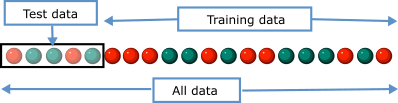
\includegraphics[width=.8\linewidth]{figures/basic_validation_EN.png}
	\end{frame}

	\begin{frame}
		\frametitle{Generalizability - Confusion Matrix}
		We can create a confusion matrix from our data!

		\centering
		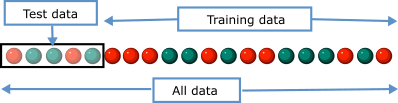
\includegraphics[width=.8\linewidth]{figures/basic_validation_EN.png}

		\begin{center}
			\begin{tabular}{|c|c|c|}
				\hline
				& \textbf{Predicted Red} & \textbf{Predicted Green} \\
				\hline
				\textbf{Actual Red} & True Green & False Green \\
				\hline
				\textbf{Actual Green} & False Red & True Red \\
				\hline
			\end{tabular}
		\end{center}
	\end{frame}

	\subsection{K-Fold Cross-Validation}
	\begin{frame}
		\frametitle{K-Fold Cross-Validation}
		But what how does selection of the test, or the train data, impact our model?  We can test that too!

		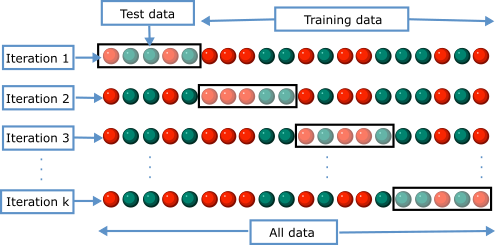
\includegraphics[width=\linewidth]{figures/K-fold_cross_validation_EN.png}
	\end{frame}

	\begin{frame}
		\frametitle{K-Fold Cross-Validation - Confusion Matrix}
		We can create a confusion matrix here too.  We simply need to calculate averages (naive, weighted) of each metric.

		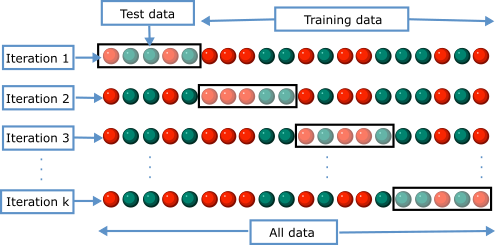
\includegraphics[width=\linewidth]{figures/K-fold_cross_validation_EN.png}
	\end{frame}

	\subsection{Stratified Cross-Validation}
	\begin{frame}
		\frametitle{Stratified Cross-Validation}
		Stratified Cross-Validation: Ensures class distribution

		This is a variation of cross-validation that ensures each fold of the validation process maintains the same proportion of classes as the complete dataset. This is particularly important when dealing with imbalanced datasets, where one class may significantly outnumber another.

    	Standard k-Fold Cross-Validation:
    	\begin{itemize}
        	\item The original dataset is randomly split into {\em k} subsets (folds).
        	\item The model is trained on {\em k-1} folds and tested on the remaining fold.
        \end{itemize}
    	
    	Stratified k-Fold Cross-Validation:
    	\begin{itemize}
        	\item The same {\em k} folds are created, but each fold is made up of roughly the same proportion of each class as the full dataset.
        	\item This ensures that if the dataset consists of 80\% class A and 20\% class B, each fold will have approximately the same ratio.
        \end{itemize}
	\end{frame}

\section{Discussion}
	\begin{frame}
		\frametitle{Group Discussion Time}
		Let's break into four groups.  Pair with someone you don't know!

		Update each other on your project, device construction, data collection, and how will you apply these metrics to assess your model(s)?
	\end{frame}

\end{document}
